\documentclass{article}
\usepackage{caption}
\usepackage{amssymb}
\usepackage{array}
\usepackage{geometry}
\usepackage{scrextend}
\usepackage{amsmath}
\usepackage{hyperref}
\usepackage{graphicx}
\usepackage{pdfpages}
\usepackage{multicol}
\usepackage{tabularx}
\usepackage{float}

\title{EE102 Homework 4}
\author{Jacob Guenther}

\geometry{
	a4paper,
	total={170mm,257mm},
	left=20mm,
	top=20mm,
}

\newcommand{\problemstatement}[3]{
\noindent
\begin{tabular}{ m{0.5cm} m{42em}}
	({#1}) & {#2}
\end{tabular}
}

\begin{document}

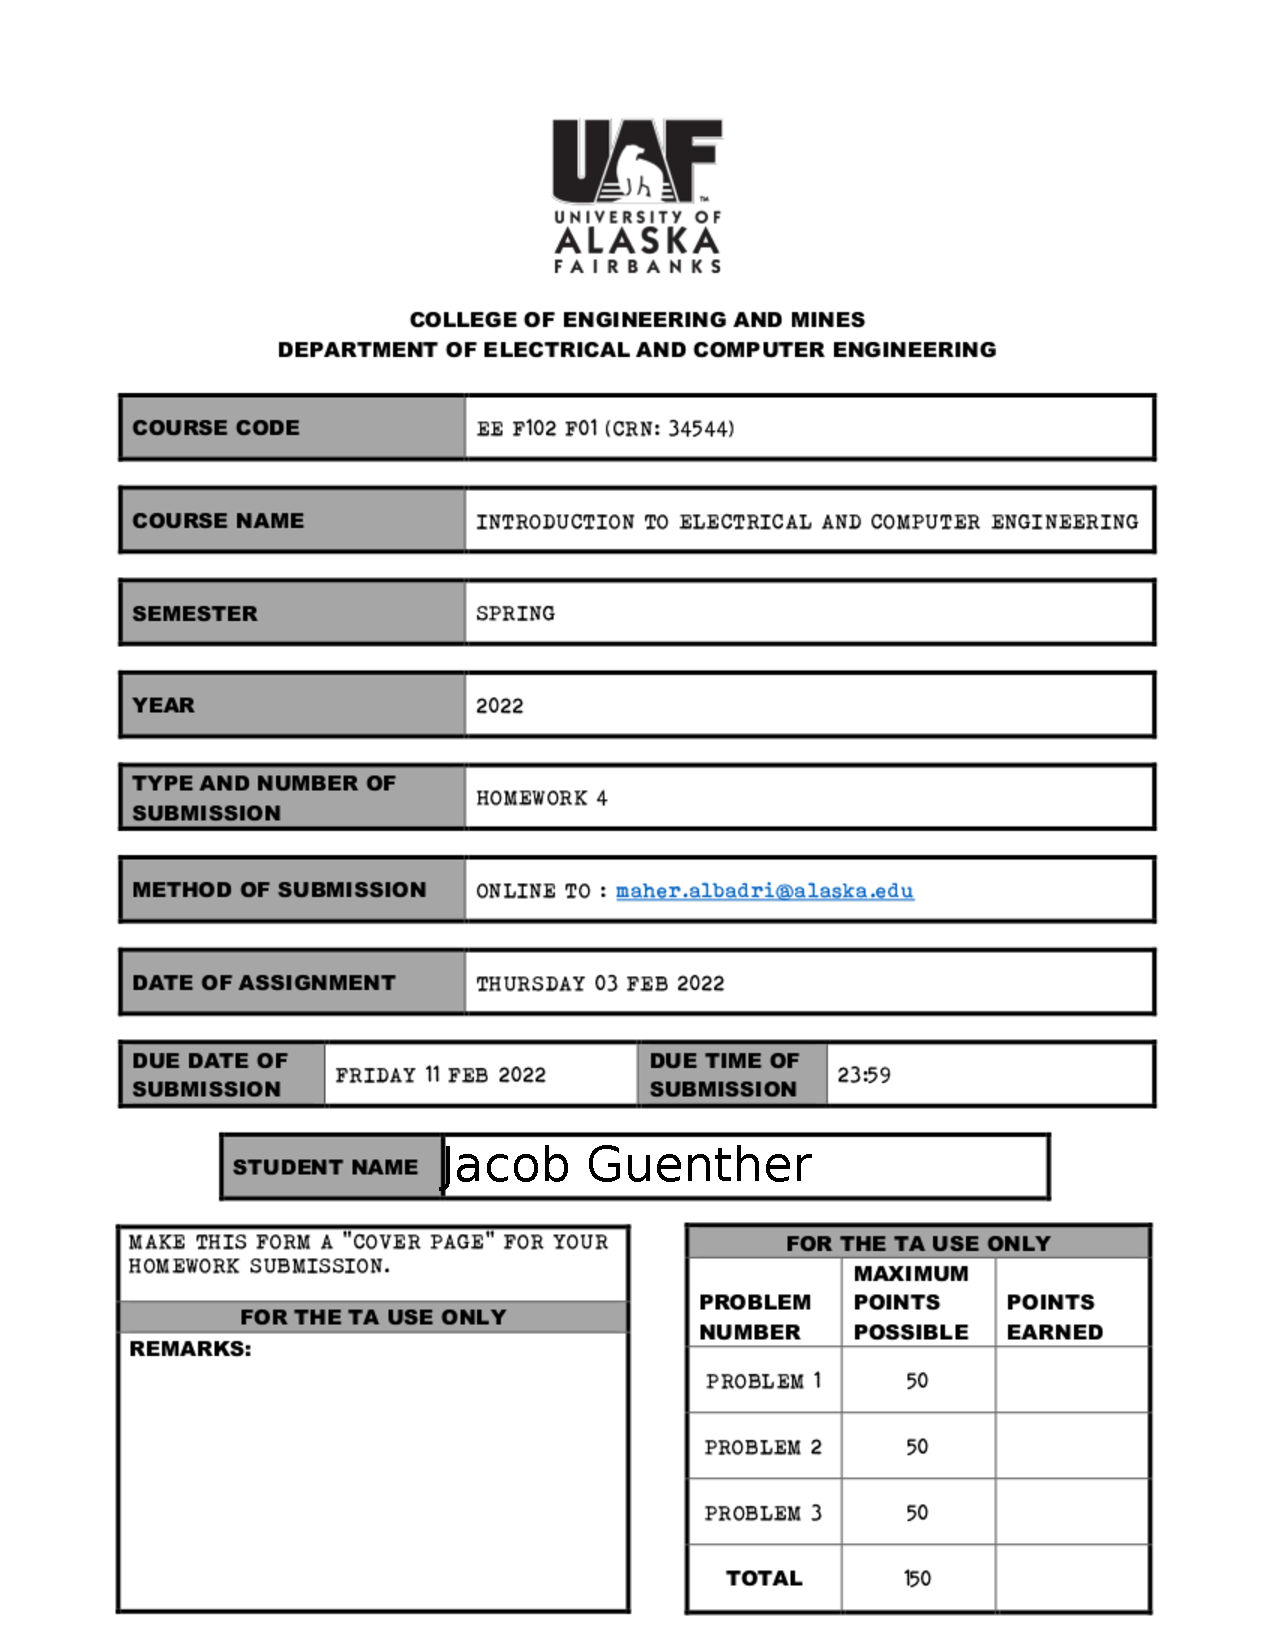
\includepdf[pages=1,pagecommand={}]{hw4_cover.pdf}

\section{Problem HW-4-1}
\problemstatement{1}{For the electric circuit shown with the given information,}{}
\begin{center}
	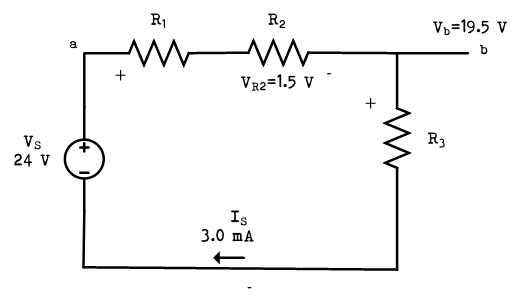
\includegraphics[width=10cm]{hw4_figure_1}
\end{center}
\begin{itemize}
	\item (a) Determine the voltage across $\text{R}_1$. \\
		\textbf{Solution:} \\
		\begin{align*}
			\text{V}_{R1} &= \text{V}_s - (\text{V}_b + \text{V}_{R1}) \\
			\text{V}_{R1} &= 24 \text{V} - (19.5 \text{V} + 1.5 \text{V}) \\
			\text{V}_{R1} &= 3 \text{V}
		\end{align*}
		\textbf{Answer:} The voltage across $\text{R}_1$ is \textbf{3 V}
	\item (b) Determine the powers $\text{P}_1$, $\text{P}_2$, $\text{P}_3$ in mW, consumed in resistors $\text{R}_1$, $\text{R}_2$, and $\text{R}_3$ respectively.
		\textbf{Note:} \\
		\begin{equation}
			\text{P} = \text{I} \cdot \text{V}
		\end{equation}
		\textbf{Solution:} \\
		\begin{align*}
			\text{P}_1 &= \text{I}_s \cdot \text{V}_{R1} \\
				&= 3.0 \text{mA} \cdot 3 \text{V} \\
				&= 9.0 \text{mW} \\
			\text{P}_2 &= \text{I}_s \cdot \text{V}_{R2} \\
				&= 3.0 \text{mA} \cdot 1.5 \text{V} \\
				&= 4.5 \text{mW} \\
			\text{P}_3 &= \text{I}_s \cdot \text{V}_{R3} \\
				&= 3.0 \text{mA} \cdot 19.5 \text{V} \\
				&= 58.5 \text{mW} \\
		\end{align*}
		\textbf{Answer:}
		\begin{itemize}
			\item $\text{P}_1$ = \textbf{9.0 mW}
			\item $\text{P}_2$ = \textbf{4.5 mW}
			\item $\text{P}_3$ = \textbf{58.5 mW}
		\end{itemize}
	\item (c) Determine the total power, in mW, supplied by the voltage source. \\
		\textbf{Solution:} \\
		\begin{align*}
			\text{P}_{total} &= \text{P}_1 + \text{P}_2 + \text{P}_3 \\
				&= 9.0 \text{mW} + 4.5 \text{mW} + 58.5 \text{mW} \\
			 	&= 71.0 \text{mW}
		\end{align*}
		\textbf{Answer:} The total power supplied is \textbf{71.0 mW}.
	\item (c) Determine the values of the resistors $\text{R}_1$, $\text{R}_2$, and $\text{R}_3$, in ohms. \\
		\textbf{Note:} \\
		\begin{equation}
			\text{R} = { \text{V} \over \text{I} }
		\end{equation}
		\textbf{Solution:} \\
		\begin{align*}
			\text{I}_s &= 3.0 \text{mA} \cdot {1 \text{A} \over 1000 \text{mA} } \\
				&= 0.003 \text{A} \\
			\text{R}_1 &= { \text{V}_{R1} \over \text{I}_s } \\
				&= { 3 \text{V} \over 0.003 \text{A} } \\
				&= 1000 \Omega \\
			\text{R}_2 &= { \text{V}_{R2} \over \text{I}_s } \\
				&= { 1.5 \text{V} \over 0.003 \text{A} } \\
				&= 500 \Omega \\
			\text{R}_3 &= { \text{V}_{R3} \over \text{I}_s } \\
				&= { 19.5 \text{V} \over 0.003 \text{A} } \\
				&= 6500 \Omega \\
		\end{align*}
		\textbf{Answer:}
		\begin{itemize}
			\item \textbf{$\text{R}_1 = \textbf{1000} \Omega$}
			\item \textbf{$\text{R}_2 = \textbf{500} \Omega$}
			\item \textbf{$\text{R}_3 = \textbf{6500} \Omega$}
		\end{itemize}
\end{itemize}

\newpage
\section{Problem HW-4-2}
\problemstatement{2}{A 30 m long copper conductor has a cross-sectional area of 0.75 $\text{cm}^2$ and its operating temperature is 35 degrees C. The temperature coefficient ($\alpha$) of the copper wire is 0.00393 per degrees C and the resistivity is $1.723 \times 10^{-8} \Omega \text{m}$.}{}
\begin{itemize}
	\item (a) Determine the total resistance of the conductor, in $\text{m} \Omega$. \\
		\textbf{Note:} \\
		\begin{equation}
			R = { \rho \cdot L \over A }
		\end{equation}
		\textbf{Solution:}
		\begin{align*}
			\text{Area} &= 0.75 \text{cm}^2 \\
			 	&= 0.75 \text{cm}^2 \cdot { 1 \text{m} \over 100 \text{cm} } \cdot { 1 \text{m} \over 100 \text{cm} } \\
			 	&= 0.000075 \text{m}^2 \\
			 \text{R} &= 1.723 \times 10^{-8} \Omega \text{m} {30 \text{m} \over 0.000075 \text{m}^2 } \\
			 	&= 0.06892 \Omega
			 \text{R} = 0.06892 \Omega \cdot { 1000 \text{m} \Omega \over 1 \Omega } \\
			 	&= 68.92 \text{m} \Omega
		\end{align*}
		\textbf{Answer:} The total resistance of the conductor is \textbf{$ \textbf{68.92 m} \Omega$}.
	\item (b) Determin the conductor resistance at 140 degrees F. \\
		\textbf{Note:} \\
		\begin{equation}
			\Delta R = k \Delta T
		\end{equation}
		\begin{equation}
			\alpha = { k \over R_{T0} }
		\end{equation}
		\begin{equation}
			^{\circ} \text{C} = {^{\circ} \text{F} - 32 \over {9 \over 5}}
		\end{equation}
		\textbf{Solution:}
		\begin{align*}
			\text{T} &= {140 ^{\circ} \text{F} - 32 \over {9 \over 5}} \\
				&= 60 ^{\circ} \text{C} \\
			\Delta \text{T} &= 60 ^{\circ} \text{C} - 35 ^{\circ} \text{C} \\
				&= 25 ^{\circ} \text{C} \\
			k &= \alpha \cdot R_{T0} \\
				&= 0.00393 \cdot { 1 \over ^{\circ} \text{C}} \cdot 0.06892 \Omega \\
				&= 0.00027086 { \Omega \over ^{\circ} \text{C} } \\
			\Delta R &= 0.00027086 { \Omega \over ^{\circ} \text{C} } \cdot 25 ^{\circ} \text{C} \\
				&= 0.0067715 \Omega \\
			\text{R}_{140F} &= \text{R} + \Delta \text{R} \\
				&= 0.06892 \Omega + 0.0067715 \Omega \\
				&= 0.0756915 \Omega \\
				&= 0.0756915 \Omega \cdot { 1000 \text{m} \Omega \over 1 \Omega } \\
				&= 75.69 \text{m} \Omega
		\end{align*}
		\textbf{Answer:} The resistance of the conductor at 140 degrees F is \textbf{$ \textbf{75.69 m} \Omega$}.
\end{itemize}

\newpage
\section{Problem HW-4-3}
\problemstatement{3}{A thermistor has the following initial data:}{}
\begin{itemize}
	\item \text{B} = 5500 \textbf{$^{\circ}$} K
	\item $\text{R}_\text{T0} = 10.5 k \Omega$
	\item $\text{T}_0$ = 29 \textbf{$^{\circ}$}C
\end{itemize}
\begin{itemize}
	\item (a) Determine the the resistance, in k$\Omega$, of the thermistor at the following temperatures: \\
	\begin{itemize}
		\item[*] $\text{T}_{1} = -20 ^{\circ} \text{C}$
		\item[*] $\text{T}_{2} = -15 ^{\circ} \text{C}$
		\item[*] $\text{T}_{3} = -10 ^{\circ} \text{C}$
		\item[*] $\text{T}_{4} = -5 ^{\circ} \text{C}$
		\item[*] $\text{T}_{5} = 0 ^{\circ} \text{C}$
		\item[*] $\text{T}_{6} = 10 ^{\circ} \text{C}$
		\item[*] $\text{T}_{7} = 20 ^{\circ} \text{C}$
		\item[*] $\text{T}_{8} = 30 ^{\circ} \text{C}$
		\item[*] $\text{T}_{9} = 40 ^{\circ} \text{C}$
		\item[*] $\text{T}_{10} = 50 ^{\circ} \text{C}$
		\item[*] $\text{T}_{11} = 100 ^{\circ} \text{C}$
	\end{itemize}
		\textbf{Note:}
		\begin{equation}
			R_{T1} = R_{T0} \cdot exp[B({1 \over T_1} - {1 \over T_0})]
		\end{equation}
		\begin{equation}
			^{\circ} \text{K} = ^{\circ} \text{C} + 217.15 
		\end{equation}
		\textbf{Solution:}
		\begin{align*}
			T_0 &= 29 ^{\circ} \text{C} \\
				&= 29 + 217.15 \\
				&= 246.15 ^{\circ} \text{K} \\
			T_1 &= -20 ^{\circ} \text{C} \\
				&= -20 + 217.15 \\
				&= 197.15 ^{\circ} \text{K} \\
			R_{T0} &= 10.5 k \Omega \\
			R_{T0} &= 10500 \Omega \\
			R_{T1} &= 10500 \Omega exp[5500 ^{\circ} \text{K} \cdot ( { 1 \over 197.15 ^{\circ} \text{K}} - { 1 \over 246.15 ^{\circ} \text{K}} )] \\
				&= 2710303.973 \Omega \\
				&= 2710303.973 \Omega \cdot { 1 \text{k} \Omega \over 1000 \Omega } \\
				&= 2710.303 \text{k} \Omega
		\end{align*}
		The rest where done in excel. \\
		\textbf{Answer:} \\
		\begin{table}[H]
			\begin{tabular}{ | c | c | r | }
			\hline
			Temperature Name &
			Temperature ($^{\circ} \text{C}$) &
			Resistance ($\text{k} \Omega$) \\
			\hline
			$\text{T}_{1}$ & $-20 ^{\circ} \text{C}$ & $2710.303 \text{k} \Omega$ \\
			\hline
			$\text{T}_{2}$ & $-15 ^{\circ} \text{C}$ & $1359.395 \text{k} \Omega$ \\
			\hline
			$\text{T}_{3}$ & $-10 ^{\circ} \text{C}$ & $704.92 \text{k} \Omega$ \\
			\hline
			$\text{T}_{4}$ & $-5 ^{\circ} \text{C}$ & $377.032 \text{k} \Omega$ \\
			\hline
			$\text{T}_{5}$ & $0 ^{\circ} \text{C}$ & $207.554 \text{k} \Omega$ \\
			\hline
			$\text{T}_{6}$ & $10 ^{\circ} \text{C}$ & $68.057 \text{k} \Omega$ \\
			\hline
			$\text{T}_{7}$ & $20 ^{\circ} \text{C}$ & $24.517 \text{k} \Omega$ \\
			\hline
			$\text{T}_{8}$ & $30 ^{\circ} \text{C}$ & $9.592 \text{k} \Omega$ \\
			\hline
			$\text{T}_{9}$ & $40 ^{\circ} \text{C}$ & $4.0373 \text{k} \Omega$ \\
			\hline
			$\text{T}_{10}$ & $50 ^{\circ} \text{C}$ & $1.913 \text{k} \Omega$ \\
			\hline
			$\text{T}_{11}$ & $100 ^{\circ} \text{C}$ & $0.0706 \text{k} \Omega$ \\
			\hline
			\end{tabular}
		\end{table}
	\item (b) Plot the resistance values (y-axis) versus temperature (x-axis). \\
		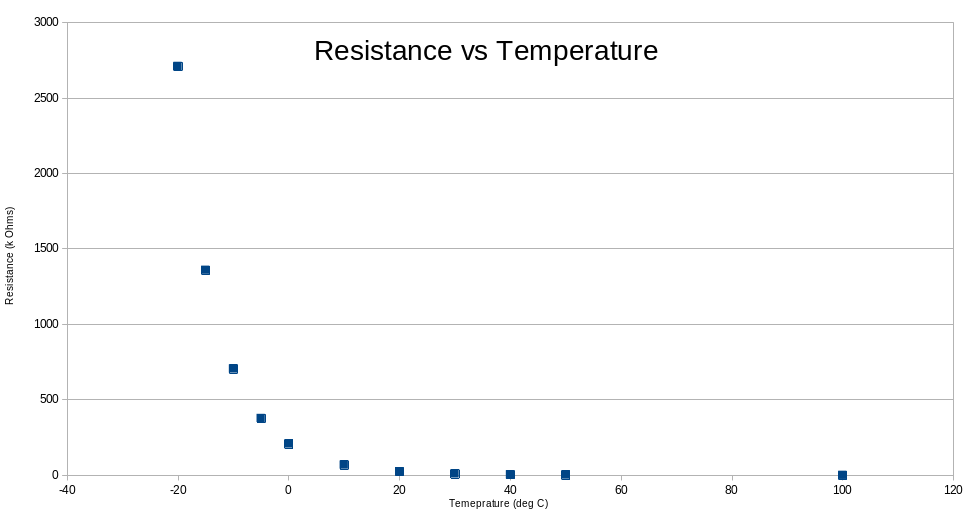
\includegraphics[width=\textwidth]{res_vs_temp}
\end{itemize}

\newpage
\section{References}
[1] Denise Thorsen, Maher Al-Badri, INTRODUCTION TO ELECTRICAL AND COMPUTER ENGINEERING, University of Alaska Fairbanks, 2022.

\end{document}